%!TEX ROOT = thesis.tex
\chapter{Symbol Error Rate (SER) for QPSK Modulation}\label{appendB}


\addcontentsline{toc}{chapter}{APPENDIX B: Symbol Error Rate (SER) for QPSK Modulation}
% % % % % % % % % % % % % % % % % % % % % % % % % % % % % % % % % % % % % % % % % % % % % % % % % %
%\captionsetup{{lofdepth=0}}
\begin{figure}[!h]
\centering
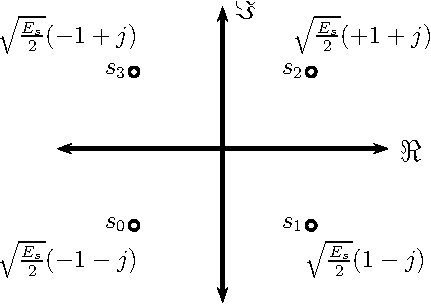
\includegraphics[width=0.5\textwidth]{./append2/QPSK_const}
%\legend{\figurename~\thefigure:~QPSK constellation.}
\caption{QPSK constellation.}
\label{figII:QPSK_const}
\end{figure}

\noindent Assuming the alphabets used for QPSK are $ \alpha_{QPSK}=\{\pm 1 \pm 1j\} $, the constellation diagram for QPSK is shown in Figure~\ref{figII:QPSK_const}. 
The factor $ \sqrt{\dfrac{E_s}{2}} $ is a normalization factor, i.e, to normalize the average energy of the transmitted symbols to 1, assuming that all symbols are equiprobable. 




	The conditional probability distribution function (PDF) of $ y $ given $ s_2 $ was transmitted (Figure~\ref{figII:Rpdf}):
	\begin{align}
	f(y/s_2)&=\dfrac{1}{\sqrt{\pi N_0}}e^{\frac{{-\big ( y-\sqrt{\frac{E_s}{2}}\big )}^2}{N_0}}
	\end{align}
	
	\begin{figure}[htb]
	%\captionsetup{list=no}
	%\stepcounter{figure}
	\centering
	\def\svgwidth{0.5\textwidth}
	\input{./append2/SER_QPSK2.pdf_tex}
	%\legend{\figurename~\thefigure:~Conditional pdf for real part (QPSK) being in error (dark area).}
	\caption{Conditional pdf for real part (QPSK) being in error (dark area).}
	\label{figII:Rpdf}
	\end{figure}
	From figure~\ref{figII:Rpdf}, symbol $ s_{2} $ is detected correctly if $ y $ falls in the hashed area, i.e.,
	\begin{equation}
	f(c|s_2)=f(\Re\{y\} > 0|s_2 )f(\Im\{y\} | s_2 )
	\end{equation}
	Probability of real part of $ y $ >$ 0 $, given $ s_2 $ was sent (i.e, dark area) is:
	\begin{align}
	f(\Re\{y\} > 0|s_2 )&=1-\dfrac{1}{\sqrt{\pi N_0}}\int\limits_{-\infty}^{0}e^{\frac{{-\big (\Re \{y\}-\sqrt{\frac{E_s}{2}}\big )}^2}{N_0}}dy\\
	&=1-\dfrac{1}{2}\text{erfc}\Big( \sqrt{\dfrac{E_s}{2N_0}} \Big)
	\end{align}
	
	Similarly, for the imaginary part of $ y $ (Figure~\ref{figII:Ipdf}):
	\begin{figure}[htb]
	%\captionsetup{list=no}
	%\stepcounter{figure}
	\centering
	\def\svgwidth{0.5\textwidth} % Defining the width since Inkscape hasn't done this yet in the .pdf_tex file
	%\small
	\input{./append2/SER_QPSK.pdf_tex}
	%\legend{\figurename~\thefigure:~Conditional pdf for imaginary part being in error (dark area).}
	\caption{Conditional pdf for imaginary part being in error (dark area).}
	\label{figII:Ipdf}
	\end{figure}
	
		\begin{align}
		f(\Im\{y\} > 0|s_2 )&=1-\dfrac{1}{\sqrt{\pi N_0}}\int\limits_{-\infty}^{0}e^{\frac{{-\big (\Im \{y\}-\sqrt{\frac{E_s}{2}}\big )}^2}{N_0}}dy\\
		&=1-\dfrac{1}{2}\text{erfc}\Big( \sqrt{\dfrac{E_s}{2N_0}} \Big)
		\end{align}
The probability of $ s_2 $ being decoded correctly is,
\begin{align}
f(c|s_2)&=\Big[ 1-\dfrac{1}{2}\text{erfc}\Big( \sqrt{\dfrac{E_s}{2N_0}} \Big)\Big]^2\\
&=\Big[ 1-\dfrac{2}{2}\text{erfc}\Big( \sqrt{\dfrac{E_s}{2N_0}} \Big)+\dfrac{1}{4}\text{erfc}^2\Big( \sqrt{\dfrac{E_s}{2N_0}} \Big) \Big]\\
&=1-\text{erfc}\Big( \sqrt{\dfrac{E_s}{2N_0}} \Big)+\dfrac{1}{4}\text{erfc}^2\Big( \sqrt{\dfrac{E_s}{2N_0}} \Big)
\end{align}

\begin{align}
P_{e,QPSK}&=1-f(c|s_2)\\
&=1-\Big[ 1-\text{erfc}\Big( \sqrt{\dfrac{E_s}{2N_0}} \Big)+\dfrac{1}{4}\text{erfc}^2\Big( \sqrt{\dfrac{E_s}{2N_0}} \Big) \Big]\\
&=\text{erfc}\Big( \sqrt{\dfrac{E_s}{2N_0}} \Big)-\dfrac{1}{4}\text{erfc}^2\Big( \sqrt{\dfrac{E_s}{2N_0}} \Big)
\end{align}

For higher values of $ E_s/N_0 $, the approximated equation is:
\begin{equation}
P_{e,QPSK} \approx \text{erfc}\Big( \sqrt{\dfrac{E_s}{2N_0}} \Big)
\end{equation}
\clearpage

